\chapter{Ewaluacja, wyniki i ograniczenia}\label{rozdz:wyniki}

\section{Jak uczciwie zmierzyć, czy model działa?}

Model zwrócił listę nut. Skąd wiemy, że jest dobra? Potrzebujemy trzech rzeczy: (i)~\emph{definicji poprawnej nuty} i miary, która łączy trafność z kompletnością (F1), (ii)~\emph{zbioru testowego}, którego model nigdy nie widział, ani w uczeniu, ani przy wyborze epoki, ani przy strojeniu progów,
(iii)~\emph{niepewności} wyniku (przedział ufności). Ten rozdział wyjaśnia wszystkie trzy, a potem podaje wyniki i --- równie ważne --- to, czego pomiar nie pokazuje.

Po tym rozdziale umiesz: (i)~policzyć precyzję, czułość i F1 z liczby trafień, (ii)~wyjaśnić, czemu średnia z F1 po nagraniach różni się od F1 policzonego razem, (iii)~policzyć błąd standardowy metodą bootstrap, (iv)~odczytać wyniki Gen~6 i wskazać ich ograniczenia.

\section{Poprawna nuta, precyzja, czułość, F1}

\haslo{dopasowanie nut}
\begin{definicja}[Trafienie]\label{def:trafienie}
Nuta przewidziana $(m,t_\mathrm{on})$ \emph{trafia} nutę wzorca $(m^\ast,t^\ast_\mathrm{on})$, gdy wysokości różnią się o mniej niż $50$ centów (czyli $m=m^\ast$ dla całkowitych numerów MIDI) i $\abs{t_\mathrm{on}-t^\ast_\mathrm{on}}\le50\ms$.
Każda nuta wzorca może być trafiona co najwyżej raz, a każda przewidziana liczy się co najwyżej raz (dopasowanie jeden do jednego; wyznacza się je algorytmem dla grafów dwudzielnych, np.\ Hopcrofta--Karpa). Dla miary \emph{z końcem} dodatkowo koniec musi się mieścić w tolerancji $\max(50\ms,\,0{,}2\,\delta)$, gdzie $\delta$ to długość nuty wzorca.
\end{definicja}

\begin{przyklad}\label{prz:trafienie}
Wzorzec ma jedną nutę $(64;\ 1{,}010)$, a model zwrócił dwie: $(64;\ 1{,}000)$ i $(64;\ 1{,}030)$. Obie są w tolerancji $50\ms$, ale dopasowanie jest jeden do jednego: jedna jest trafieniem (TP), druga fałszywym alarmem (FP). Gdyby model nie zwrócił nic, nuta wzorca byłaby pominięta (FN).
\end{przyklad}

Niech $\mathrm{TP}$ będzie liczbą trafień, $\mathrm{FP}$ liczbą przewidzianych niezatrafionych, $\mathrm{FN}$ liczbą pominiętych nut wzorca. Wtedy
\begin{equation}
  P=\frac{\mathrm{TP}}{\mathrm{TP}+\mathrm{FP}}\ \text{(precyzja)},\qquad R=\frac{\mathrm{TP}}{\mathrm{TP}+\mathrm{FN}}\ \text{(czułość)},\qquad F_1=\frac{2PR}{P+R}.
\end{equation}

\begin{twierdzenie}[Postać F1 i położenie między $P$ i $R$]\label{tw:f1}
Przy $\mathrm{TP}>0$: $F_1=\dfrac{2\,\mathrm{TP}}{2\,\mathrm{TP}+\mathrm{FP}+\mathrm{FN}}$ oraz $\min(P,R)\le F_1\le\max(P,R)$.
\end{twierdzenie}
\begin{pomyslDowodu}
F1 to średnia harmoniczna $P$ i $R$; po wstawieniu ułamków licznik i mianownik upraszczają się do liczb zliczeń. Nierówność wynika z tego, że średnia harmoniczna leży między składnikami.
\end{pomyslDowodu}
\begin{proof}
Niech $a=\mathrm{TP}+\mathrm{FP}$ i $b=\mathrm{TP}+\mathrm{FN}$, więc $P=\mathrm{TP}/a$, $R=\mathrm{TP}/b$.
\begin{align*}
F_1 &= \frac{2\,\frac{\mathrm{TP}}{a}\frac{\mathrm{TP}}{b}}{\frac{\mathrm{TP}}{a}+\frac{\mathrm{TP}}{b}} && \pow{(def.)}\\
 &= \frac{2\,\mathrm{TP}^2}{\mathrm{TP}\,(a+b)}=\frac{2\,\mathrm{TP}}{a+b} && \pow{(mnożenie przez $ab$, skrócenie $\mathrm{TP}$)}\\
 &= \frac{2\,\mathrm{TP}}{2\,\mathrm{TP}+\mathrm{FP}+\mathrm{FN}}. && \pow{($a+b$ rozpisane)}
\end{align*}
Dla nierówności załóżmy $P\le R$ (drugi przypadek jest symetryczny): $F_1=\dfrac{2PR}{P+R}\ge\dfrac{2PR}{2R}=P$, bo $P+R\le2R$; oraz $F_1\le\dfrac{2PR}{2P}=R$, bo $P+R\ge2P$. To kończy dowód.
\end{proof}

W zwykłym języku: F1 zlicza trafienia podwójnie i dzieli przez sumę „wszystkiego, co się liczyło” --- trafień, fałszywych alarmów i pominięć. Nie da się mieć dobrego F1 ani przez mówienie bardzo mało (wysokie $P$, niskie $R$), ani przez mówienie bardzo dużo (odwrotnie).

\begin{figure}[ht]
\centering
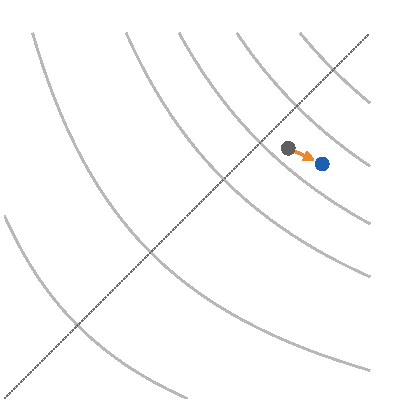
\includegraphics[width=\linewidth]{figures/f1-poziomice.pdf}
\sidecaption{Płaszczyzna precyzja (poziom) -- czułość (pion), od $0{,}5$ do $1$, z poziomicami F1 (szare linie, od $0{,}6$ do $0{,}95$; kropkowana to $P=R$). Szara kropka: dekoder domyślny ($P=88{,}8\%$, $R=84{,}2\%$), niebieska: dostrojony ($93{,}5\%$, $82{,}1\%$); strzałka pokazuje zmianę.
Precyzja rośnie o $4{,}7$ punktu, czułość spada o $2{,}1$, a punkt przechodzi na wyższą poziomicę (F1 ze średnich $P,R$: $86{,}5\%\to87{,}4\%$); F1 jest tym większe, im bliżej górnego prawego rogu i im bliżej przekątnej. Raportowane makro-F1 ($85{,}9\%\to86{,}6\%$) jest liczone inaczej (przykład~\ref{prz:makro-mikro}). \label{rys:f1-poziomice}}
\end{figure}

\begin{naliczbach}
Model na teście (średnie): $P=88{,}84\%$, $R=84{,}25\%$. Gdyby policzyć $F_1$ z tych dwóch średnich, wyszłoby $2PR/(P+R)=86{,}5\%$. Tymczasem raportowane F1 nut ma $85{,}94\%$ --- mniej. Różnica nie jest błędem: to \emph{średnia z F1 po nagraniach} (makro), a nie F1 ze średnich.
\end{naliczbach}

\begin{przyklad}[Makro i mikro]\label{prz:makro-mikro}
Dwa nagrania: A ma $\mathrm{TP}=9$, $\mathrm{FP}=1$, $\mathrm{FN}=1$ ($F_1=0{,}9$), B ma $\mathrm{TP}=1$, $\mathrm{FP}=3$, $\mathrm{FN}=3$ ($F_1=0{,}25$). \emph{Makro} (średnia z F1): $(0{,}9+0{,}25)/2=0{,}575$.
\emph{Mikro} (zsumowane zliczenia $\mathrm{TP}=10$, $\mathrm{FP}=4$, $\mathrm{FN}=4$): $F_1=20/28=0{,}714$. Mikro daje większą wagę nagraniom z większą liczbą nut; makro traktuje każde nagranie jednakowo. W książce podajemy makro, chyba że napisano inaczej.
\end{przyklad}

\section{Niepewność: bootstrap}

Test ma $700$ nagrań; wynik zależy od tego, które to nagrania. \emph{Bootstrap} szacuje tę zależność: losujemy ze zwracaniem $n$ nagrań z $n$ dostępnych, liczymy średnią, powtarzamy wiele razy i patrzymy na rozrzut.

\begin{twierdzenie}[Wariancja średniej bootstrapowej]\label{tw:bootstrap}
Niech $x_1,\dots,x_n$ będą wynikami (np.\ F1) $n$ nagrań, $\bar x$ ich średnią, a $\bar x^\ast$ średnią z $n$ losowań ze zwracaniem. Wtedy $\Exp[\bar x^\ast]=\bar x$ oraz
\begin{equation}
  \Var(\bar x^\ast)=\frac{\hat\sigma^2}{n},\qquad\hat\sigma^2=\frac1n\sum_{i=1}^n(x_i-\bar x)^2.
\end{equation}
\end{twierdzenie}
\begin{pomyslDowodu}
Każde losowanie to niezależna zmienna o rozkładzie równomiernym na $\{x_1,\dots,x_n\}$; średnia $n$ takich zmiennych ma średnią $\bar x$ i wariancję równą wariancji pojedynczego losowania podzielonej przez $n$.
\end{pomyslDowodu}
\begin{proof}
Niech $X_1^\ast,\dots,X_n^\ast$ będą niezależnymi losowaniami z $\{x_i\}$, każde z prawdopodobieństwem $1/n$. Wtedy
\begin{align*}
\Exp[X_j^\ast] &= \frac1n\sum_ix_i=\bar x, && \pow{(def.\ wartości oczekiwanej)}\\
\Var(X_j^\ast) &= \frac1n\sum_i(x_i-\bar x)^2=\hat\sigma^2, && \pow{(def.\ wariancji)}\\
\Var(\bar x^\ast) &= \frac1{n^2}\sum_{j=1}^n\Var(X_j^\ast)=\frac{\hat\sigma^2}{n}. && \pow{(niezależność)}
\end{align*}
Średnia ma więc dokładnie wariancję $\hat\sigma^2/n$, czyli odchylenie standardowe maleje jak $1/\sqrt n$: czterokrotnie więcej nagrań zmniejsza niepewność o połowę. To kończy dowód.
\end{proof}

\begin{naliczbach}
Dla sześciu wyników $x=(84,88,90,79,91,86)$: $\bar x=86{,}33$, $\hat\sigma^2=16{,}22$, więc błąd standardowy $\sqrt{16{,}22/6}=1{,}644$. Symulacja bootstrap ($2\cdot10^5$ powtórzeń) daje $1{,}645$ i $95\%$ przedział percentylowy $[82{,}8;\ 89{,}3]$. Przedział $95\%$ to ok.\ $\pm2$ błędy standardowe.
\end{naliczbach}

Gdy porównujemy dwa warianty (np.\ dekoder domyślny i dostrojony), stosujemy \emph{sparowany} bootstrap: losujemy te same indeksy nagrań dla obu wariantów i bootstrapujemy \emph{różnicę} wyników. Szum związany z trudnością nagrań (wspólny dla obu wariantów) wtedy się znosi, i przedział różnicy jest wąski: np.\ F1 nut $+0{,}64$ z przedziałem $[0{,}46;\ 0{,}83]$ (rozdział~\ref{rozdz:dekoder}).

\begin{pulapka}
Przedział ufności bootstrap opisuje niepewność związaną z \emph{doborem nagrań testowych}, nie z innymi źródłami błędu: z tym, że dane są syntetyczne, że inny mikrofon da inny wynik, że model był uczony tylko raz (jedno ziarno). Wąski przedział nie znaczy, że wynik przeniesie się na inne dane.
\end{pulapka}

\section{Wyniki Gen~6}

Test: $700$ nagrań, w tym $180$ prawdziwej gitary (GuitarSet, gracze $03$--$05$) i $520$ syntezy klasyki; wszystkie utwory i gracze nieobecni w uczeniu (rozdział~\ref{rozdz:dane}). Wszystkie miary liczy ten sam moduł, zgodny z biblioteką \texttt{mir\_eval} do $10^{-9}$.

\begin{table}[ht]
\centering\small
\begin{tabular}{@{}lccc@{}}
\toprule
miara (makro, $700$ nagrań) & dekoder domyślny & dekoder dostrojony & zmiana (95\%)\\
\midrule
F1 nut & $85{,}9\ [85{,}0;\,86{,}8]$ & $\mathbf{86{,}6}$ & $+0{,}64\ [0{,}46;\,0{,}83]$\\
F1 nut z końcem & $69{,}4\ [67{,}9;\,71{,}0]$ & $\mathbf{70{,}0}$ & $+0{,}59\ [0{,}32;\,0{,}85]$\\
F1 klatkowe & $88{,}5\ [87{,}9;\,89{,}1]$ & $87{,}3$ & $-1{,}29\ [-1{,}50;\,-1{,}10]$\\
precyzja / czułość nut & $88{,}8\ /\ 84{,}2$ & $93{,}5\ /\ 82{,}1$ & ---\\
\bottomrule
\end{tabular}
\caption{Wyniki Gen~6 (model z epoki $81$) na zbiorze testowym. Źródło: \texttt{docs/WYNIKI.md}.}
\label{tab:wyniki-test}
\end{table}

\begin{table}[ht]
\centering\small
\begin{tabular}{@{}lccc@{}}
\toprule
GuitarSet $03$--$05$ & Gen~5 & Gen~6 (końcowy) & Gen~6 + dostrojony dekoder\\
\midrule
F1 nut razem & $79{,}5$ & $87{,}2$ & ---\\
akompaniament / melodie & $75{,}6\ /\ 83{,}4$ & $85{,}1\ /\ 89{,}2$ & $87{,}3\ /\ 90{,}7$ (makro)\\
nuty z końcem, razem & $40{,}9$ & $74{,}8$ & ---\\
\bottomrule
\end{tabular}
\caption{Gen~5 i Gen~6 na prawdziwej gitarze (GuitarSet, gracze $03$--$05$). Liczby Gen~5 pochodzą z opisu projektu (ten sam podział, wcześniejszy kod oceny), więc porównanie jest przybliżone. Tabulatura (Gen~6, mikro): akompaniament --- F1 par struna--próg $82{,}2\%$, trafna struna $91{,}3\%$, TDR $91{,}7\%$; melodie --- $75{,}1\%$, $83{,}2\%$, $84{,}6\%$.}
\label{tab:gen5-gen6}
\end{table}

\begin{figure*}[ht]
\centering
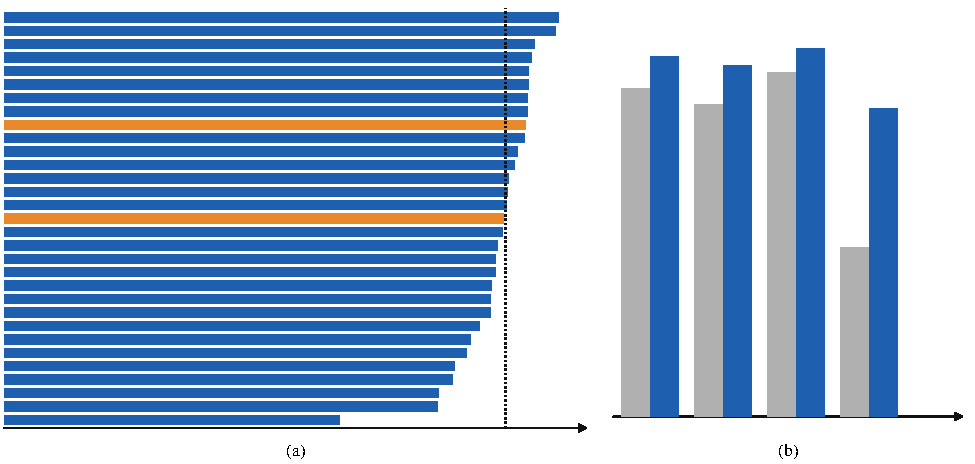
\includegraphics[width=\linewidth]{figures/wyniki-grupy.pdf}
\caption{(a) F1 nut (makro) dla każdej z $31$ grup testowych modelu końcowego (dekoder domyślny), od najlepszej do najgorszej; pomarańczowe słupki to prawdziwa gitara (GuitarSet), niebieskie --- syntetyczne nagrania klasyki; kropkowana pionowa to wynik ogólny $85{,}94\%$.
Najlepsze: pizzicato ($95{,}0\%$), ukulele ($94{,}5\%$), gitara klasyczna ($90{,}9\%$, $n=74$); najsłabsze: chór ($57{,}5\%$), wiolonczela ($74{,}3\%$), syntezator ($74{,}3\%$). (b) Gen~5 (szare) i Gen~6 (niebieskie) na GuitarSet: F1 nut razem, akompaniament, melodie, nuty z końcem (od lewej).}
\label{rys:wyniki-grupy}
\end{figure*}

\textbf{Jak to czytać.} Najlepiej wypadają instrumenty o szarpanym, wyraźnym początku (pizzicato, ukulele, gitara): tolerancja $50\ms$ jest dla nich łatwa. Najgorzej --- chór, smyczki, instrumenty z wibrato i rozmytym początkiem: tam sam początek nuty jest niejednoznaczny
nawet dla człowieka, a bogate alikwoty utrudniają odróżnienie nut. Wzorzec zgadza się z fizyką problemu (rozdziały~\ref{rozdz:alikwoty} i \ref{rozdz:fourier}). Grupy z kilkoma nagraniami ($n<12$) są niepewne.

Szybkość: dla nagrania $39$ s na $4$ rdzeniach CPU cechy zajmują $1{,}9$ s, sieć $2{,}1$ s, razem $4{,}0$ s, czyli \emph{$0{,}10$ czasu nagrania} (na $1$ rdzeniu $0{,}30$): trzy minuty gry to ok.\ $19$ s na $4$ rdzeniach.

\section{Co ten pomiar \emph{nie} pokazuje}

Uczciwa lista ograniczeń (część to wnioski wprost z dokumentacji projektu):
\begin{enumerate}
\item \textbf{Dane syntetyczne.} Tylko GuitarSet ($168$ nagrań uczących) to prawdziwa gitara; kolejne sesje uczenia dołożyły głównie syntezę i na GuitarSet dały najmniej ($+0{,}4$ i $+0{,}7$ punktu). Dokładność dla gitary z innym mikrofonem, pomieszczeniem czy przetwornikiem piezo jest \emph{niezmierzona}.
\item \textbf{Brak badań ablacyjnych.} Nie zmierzono osobno wpływu bloków harmonicznych, uwagi między wysokościami, poszczególnych augmentacji ani długości uczenia. Poprawa Gen~5$\to$Gen~6 jest łączna (cechy, architektura, dane, głowice). Teza, że uwaga między wysokościami ogranicza błędy oktawowe, jest \emph{motywacją projektową}, nie wynikiem eksperymentu.
Błąd oktawowy pozostaje wysoki: $24{,}4\%$ fałszywych alarmów klatkowych leży oktawę od prawdziwej nuty.
\item \textbf{Głośność.} Głowica głośności jest nieuczona (żadne źródło nie ma etykiet).
\item \textbf{Progi dekodera} zostały dobrane na małej walidacji ($222$ nagrania, w tym tylko $12$ prawdziwej gitary); zysk na teście ($+0{,}64$) jest o połowę mniejszy niż na walidacji ($+1{,}30$).
\item \textbf{Wybór epoki} odbył się na walidacji, która zawiera tylko $12$ nagrań GuitarSet --- niewielkie ryzyko dopasowania do walidacji.
\item \textbf{Nie sprawdzono} trybu przyczynowego (analizy na żywo) ani działania po przeniesieniu wag do silnika C++/WebAssembly (jest zaplanowane).
\item \textbf{Jedno uruchomienie uczenia} (jedno ziarno losowości): nie znamy zmienności wyniku między powtórzeniami uczenia.
\end{enumerate}

\begin{intuicja}
Dobra ewaluacja to nie tylko duża liczba, ale też jasne granice jej ważności. Wynik $86{,}6\%$ znaczy: \emph{na tych} $700$ nagraniach, \emph{z tym} dekoderem, \emph{przy tej} tolerancji i \emph{tym} podziale. Każda z tych części jest założeniem, które trzeba pamiętać, mówiąc, że „model działa”.
\end{intuicja}

\section*{Podsumowanie}
\begin{itemize}
\item Trafienie: ta sama wysokość i początek w $\pm50\ms$, dopasowanie jeden do jednego; $F_1=2\mathrm{TP}/(2\mathrm{TP}+\mathrm{FP}+\mathrm{FN})$ leży między $P$ i $R$ (tw.~\ref{tw:f1}).
\item Średnia z F1 po nagraniach (makro) nie jest F1 ze średnich $P$ i $R$ (przykład~\ref{prz:makro-mikro}).
\item Bootstrap: $\Var(\bar x^\ast)=\hat\sigma^2/n$ (tw.~\ref{tw:bootstrap}); porównania robimy sparowanym bootstrapem.
\item Gen~6 na $700$ niewidzianych nagraniach: F1 nut $85{,}9\%$ ($86{,}6\%$ z dostrojonym dekoderem); na GuitarSet $87{,}3\,/\,90{,}7\%$ (akompaniament/melodie) wobec $75{,}6\,/\,83{,}4\%$ w Gen~5 (porównanie przybliżone).
\item Ograniczenia: głównie dane syntetyczne, brak ablacji, jedno ziarno, niezmierzona gitara w innych warunkach.
\end{itemize}

\begin{sprawdz}
\begin{enumerate}
\item Model zwrócił $50$ nut, z czego $40$ trafiło; wzorzec miał $60$ nut. Policz $P$, $R$, $F_1$ i sprawdź wzór z tw.~\ref{tw:f1}.
\item Nagranie ma $\mathrm{TP}=18$, $\mathrm{FP}=2$, $\mathrm{FN}=6$. Ile wynosi $F_1$? Co się stanie z $F_1$, gdy zmienimy próg dekodera tak, że $\mathrm{FP}$ spadnie do $0$, ale $\mathrm{TP}$ spadnie do $15$ (a $\mathrm{FN}$ wzrośnie do $9$)?
\item Dla $n=10$ wyników z $\hat\sigma=5$ policz błąd standardowy bootstrap. Ile nagrań trzeba, żeby był o połowę mniejszy?
\item Dlaczego sparowany bootstrap daje węższy przedział różnicy niż porównanie dwóch niezależnych przedziałów?
\end{enumerate}
\end{sprawdz}

\subsection*{Rozwiązania}
\begin{enumerate}
\item $P=40/50=0{,}8$, $R=40/60=0{,}667$, $F_1=2\cdot0{,}8\cdot0{,}667/(1{,}467)=0{,}727$; ze wzoru $2\cdot40/(80+10+20)=80/110=0{,}727$. \checkmark
\item $F_1=36/(36+2+6)=36/44=0{,}818$. Po zmianie: $F_1=30/(30+0+9)=30/39=0{,}769$ --- spadek: precyzja wzrosła do $1$, ale czułość spadła z $0{,}75$ do $0{,}625$; zmiana, która poprawia jedną z miar kosztem drugiej, nie musi poprawić F1.
\item $\hat\sigma/\sqrt n=5/\sqrt{10}=1{,}58$; żeby błąd był o połowę mniejszy, trzeba $4\times$ więcej nagrań, czyli $n=40$ ($5/\sqrt{40}=0{,}79$).
\item Obie wersje liczone są na tych samych nagraniach, więc „trudność” nagrania (wspólny składnik) wpływa na oba wyniki podobnie i znosi się w różnicy; różnica ma mniejszą wariancję niż suma wariancji niezależnych szacunków.
\end{enumerate}
